\documentclass[10pt]{article} % use larger type; default would be 10pt

\usepackage[utf8]{inputenc} % set input encoding (not needed with XeLaTeX)
\usepackage[english]{babel}

%%% Examples of Article customizations
% These packages are optional, depending whether you want the features they provide.
% See the LaTeX Companion or other references for full information.

%%% PAGE DIMENSIONS
\usepackage{geometry} % to change the page dimensions
\geometry{a4paper} % or letterpaper (US) or a5paper or....
\geometry{margin=1.5in,lmargin=0.75in,rmargin=0.75in} % for example, change the margins to 2 inches all round
% \geometry{landscape} % set up the page for landscape
%   read geometry.pdf for detailed page layout information

\usepackage{graphicx} % support the \includegraphics command and options
\usepackage{wrapfig}

\usepackage{xcolor}

\usepackage[parfill]{parskip} % Activate to begin paragraphs with an empty line rather than an indent

%%% PACKAGES
\usepackage{booktabs} % for much better looking tables
\usepackage{array} % for better arrays (eg matrices) in maths
\usepackage{paralist} % very flexible & customisable lists (eg. enumerate/itemize, etc.)
\usepackage{verbatim} % adds environment for commenting out blocks of text & for better verbatim
\usepackage{subfig} % make it possible to include more than one captioned figure/table in a single float
% These packages are all incorporated in the memoir class to one degree or another...

\usepackage{listings}

%%% TILTLE AND AUTHOR

\title{
	Predictive Text
}


\author{Y3839090}
%\date{} % Activate to display a given date or no date (if empty),
         % otherwise the current date is printed 
\makeatletter

%%% HEADERS & FOOTERS
\usepackage{fancyhdr} % This should be set AFTER setting up the page geometry
\pagestyle{fancy} % options: empty , plain , fancy
\renewcommand{\headrulewidth}{1pt} % customise the layout...
\lhead{\@title}\chead{}\rhead{\@author}
\lfoot{}\cfoot{\thepage}\rfoot{}

%%% SECTION TITLE APPEARANCE
\usepackage{sectsty}
\allsectionsfont{\sffamily\mdseries\upshape} % (See the fntguide.pdf for font help)
% (This matches ConTeXt defaults)

%%% ToC (table of contents) APPEARANCE
\usepackage[nottoc,notlof,notlot]{tocbibind} % Put the bibliography in the ToC
\usepackage[titles,subfigure]{tocloft} % Alter the style of the Table of Contents
\renewcommand{\cftsecfont}{\rmfamily\mdseries\upshape}
\renewcommand{\cftsecpagefont}{\rmfamily\mdseries\upshape} % No bold!

% biblatex for citations
\usepackage{csquotes}
\usepackage[
backend=biber,
style=numeric,
sorting=ynt
]{biblatex}
\addbibresource{references.bib}
\usepackage{url}

\usepackage[colorlinks=false,
            allbordercolors={0 0 0},
            pdfborderstyle={/S/U/W 1}]{hyperref}


\graphicspath{{Images/}}

%%% END Article customizations

%%% The "real" document content comes below...


\begin{document}
    
	\begin{titlepage}
		\centering
		
\includegraphics[width=0.5\textwidth]{UoY_logo}\par\vspace{1cm}
		{\scshape\LARGE Department of Electronics \par}
		\vspace{1cm}
		{\scshape\Large Data Structures and Algorithms Assessment \par}
		\vspace{2cm}
		{\huge\bfseries Predictive Text\par}

		% maybe an image here
	
		\vfill
		{\Large\itshape \@author \par}
		\vspace{2cm}
		{\large \today\par}
	\end{titlepage}
	
	\pagenumbering{roman} % Start roman numbering
	
	\tableofcontents
	\newpage
	
	\pagenumbering{arabic} % Start roman numbering
	
	\section{What is a predictive text system and how do they work?}
		In order to create a predictive text system, their behaviour has to be understood.
		
		A predictive text system's (also known as  auto-complete or word completion) role is to take a partial word and return a list of suggestions. They use some form of dictionary of known words to offer these suggestions.
		\subsection{How users interact with predictive text systems.}
			Users interact with predictive text systems via some kind of text input device. Most users interact with some kind of predictive text system on a daily basis on either their PC or mobile device. The UI for both desktop and mobile devices follow the same basic pattern. The user begins by entering text normally via a keyboard or touch screen and once there are a sufficient number of letters for the system to make a reasonable guess (often two letters), the system presents the user with a list of predicted words. The user is then able to press a key to select which of the suggestions they want to use or continue typing and ignore the systems suggestions. The suggested word replaces the partial word they were typing so that they can move on the the next word.
		\subsection{The behaviour of predictive text systems.}
			Predictive text system often return result that fall into a few broad categories.
			\begin{description}
				\item [The input.] One of the options in a predictive text system is always to keep the partial word that you already have. This is often achieved by returning the input as one of the items in the suggestion list. This behaviour can also happen if the partial word is actually a valid word from the predictive text systems dictionary.
				\item [A word prefixed by the partial word.] The most common results from predictive text systems are words that are prefixed by the partial word the user has entered. An example of this is that ``hel" may return ``hel\textit{p}", ``hel\textit{l}" or ``hel\textit{lo}". 
				\item [A word that shares a prefix with the partial word.] An example of this is that ``applez" may return ``apple", ``apples" or``app". 
			\end{description}
			
			More sophisticated system may also use frequency analysis techniques, lexicographical distance algorithms and consider context to make smarter suggestions. These are out side of the scope of this project ( Our dictionary doesn't contain any frequency data or phrase data).

	\section{Requirements}
		Now that a predictive text systems behaviour has been defined, a set of success criteria can be derived.
		\begin{enumerate}
			\item The system must use ISO C99/C11 C (``ANSI C") .
			\item The system must compile with minGW (gcc)
			\item The system must compile and execute correctly on the university lab machines in PT108.
			\item The system must load a word dictionary from file. \textit{(provided file words.txt)}
			
			\item The system must be capable of adding the loaded words into a data structure to store them whilst the program is running
			\item The system must store these words in a space efficient data structure.
			\item The system must be able to access these words in a time efficient manner.
			
			\item The system must be able to check to see if a partial word is contained in that data structure.
			\item The system must be able to check to see if a partial word that is stored in the data structure is a complete word from the dictionary.
			\item The system must be able to make suggestions of words that are prefixed by a partial word.
			\item The system must be able to make suggestions of words that share a common prefix with a partial word.
			
			\item The system must let the user enter a string of text.
			\item The system must be able to present the user with a suggestion mode where they will be presented with a set of suggestions which they can chose between.
			
			\item The system should let the user select the one of these suggestions.
			\item The system should replace the partial word with the selected word.
			\item The system should let the user delete characters with backspace.

			\item The system could be extended to deal with punctuation.
			\item The system could be extended to deal with Capitalisation.
			\item The system could present the users with suggestions as they are typing.
			
		\end{enumerate}
	\section{Data Structures}
		A predictive text program needs a to be able to access a set of common words.
		 Storing and accessing these words efficiently is one of the challenges in creating a fast predictive text engine.
		  I decided to use a trie\cite{book:ADS:trie} structure.
		  
		\subsection{Trie}
			\subsubsection{What is a trie}
			
				\begin{wrapfigure}{r}{0.33\textwidth} %this figure will be at the right
    				\centering
    				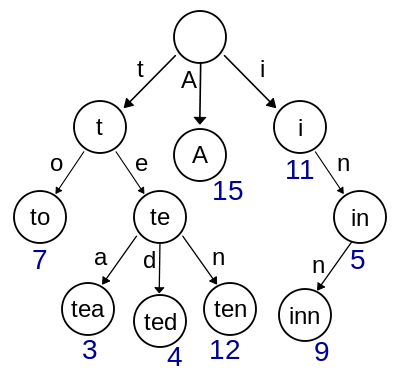
\includegraphics[width=0.33\textwidth]{Trie_example}
    				\caption{A trie for keys "A", "to", "tea", "ted", "ten", "i", "in", and "inn" \cite{fig:Trie_example}. }
    				\label{fig:Trie_example}
				\end{wrapfigure}
				
				The trie is a tree-like data structure often used for storing strings. Each node in the trie represents a single letter in a string. Each node in a trie has a fixed number of child nodes like a binary search tree. Unlike the binary search tree the trie does not have two child nodes, it has one for each letter of the alphabet. This allows the trie nodes to not store their value because their position determines it. A node's children share a common prefix, that prefix is the value of there parent node.

                There are many features of tries that make them a good choice for a predictive text system. One of them is that values can be look up by their prefixes. Predictive text systems use a partial word (a prefix) to search for possible full words. So it's important that prefix look-ups are fast and efficient. [TODO:: ADD MORE STUFF HERE]
				
			\subsubsection{Time complexity of a trie}
			    Tries are structure in such a way that they perform look ups rather than searches.
			
				The look up time for a value in a trie is dependant upon \begin{math}len(string)\end{math}, where \begin{math}len(string)\end{math} is the length of the word to look up\cite{book:ADS:complexity}. This gives the trie a \begin{math} O(1) \end{math} search time in regards to \begin{math} n \end{math} (the number of words). Meaning that searches in a trie do not depend on the number of items in the trie. A predictive text function relies upon look ups. Every time a user presses a key the system will preform at least one look up and so it is vital that these searches be fast. 
				
				The time complexity of deletion in a trie is also linear. Deletions time complexity is 
				\begin{math}\vert A \vert * len(string)\end{math}, where \begin{math}len(string)\end{math} is the length of the word to look up and \begin{math}\vert A \vert \end{math} is the size of the alphabet\cite{book:ADS:complexity}.
				This is also a \begin{math} O(1) \end{math} operation.
				In the use case as a Predictive text engine deletions will be very rare or non-existent.
				A simple implementation of predictive text may not allow the user to delete words form the dictionary at all. 
				
				The time complexity of insertion in a trie is the same as for deletions. Insertion time complexity is \begin{math}\vert A \vert  * len(string))\end{math}, where \begin{math}len(string)\end{math} is the length of the word to look up and \begin{math}\vert A \vert \end{math} is the size of the alphabet\cite{book:ADS:complexity}.
				This, again, is a \begin{math} O(1) \end{math} operation.
				When used in a predictive text engine most of the insertion into the trie will be made when loading the dictionary from file. 
				
			\subsubsection{Space complexity of a trie}
			    The space complexity of a trie is \begin{math} \vert A \vert \Sigma_i len(w_i)\end{math} where there are strings \begin{math} w_0 \end{math} to \begin{math} w_n \end{math} and \begin{math}\vert A \vert \end{math} is the size of the alphabet \cite{book:ADS:complexity}.
			    This is saying that the space complexity of a trie is equal to the size of the alphabet by the total length of all the strings.
			    Expressed in therms of \begin{math} n \end{math} this becomes \begin{math} \vert A \vert * n * l \end{math} where \begin{math}\vert A \vert \end{math} is the size of the alphabet and \begin{math} l \end{math} is the average length of the words.
			    In this form it is easy to see that the space required to store is governed by a  \begin{math} O(n) \end{math} relationship ship.
			    
            \subsubsection{Space vs Time}
                The tire data structure sacrifices a good space complexity for time complexity that doesn't depend on the number of strings that it is storing. 
                
		\subsection{Alternative Data structures}
		    This section details some alternative data structures that were be considered for storing the word list.
		    
			\subsubsection{Binary Search Trees vs Tries}
			    Both BST (Binary search trees) and Tries are ordered trees.
			    Unlike tries each node in a BST contains a maximum of 2 children. All of a nodes children on the 'left' side have a smaller value than the node and all the nodes on the right have a large value (identical values are normal omitted from BST). BST differ from tries in that each node in a BST stores a value.
			    
			    When considering space complexity BST can be shown to have a complexity of \begin{math}O(n)\end{math} \cite{book:BST:complexity}. 
			    The big-O space complexity of a trie and BST is the same.
			    
			    When considering search speed Tries are much faster than BST. For a balanced binary search tree the average time complexity of a search is \begin{math} O(n) \end{math}. This is much worse than the trie's \begin{math} O(1) \end{math} time complexity.
			    
			    Predictive text systems preform look ups via prefixes. Binary search trees don't offer any particular advantage in this area whilst tries do (All children of a node are prefixed by that node).
			    
			    It is also worth noting that BST require a lot of comparisons. Comparisons of two strings is not an atomic operation and its worst case time complexity is \begin{math}O(l)\end{math}, where \begin{math}l\end{math} is the length of the string.
			    
			    Trie are a better choice for the purpose of a predictive text system. 
			    
			\subsubsection{Hash Table vs Tries}
			    Hash tables are an associative data structure where a key can be used to look up a value and the value is used to generate the key.
			    
			    They require the use of a hash function which are proportional to the length of the input string, not constant time.
			    
			    The space complexity of a hash map is \begin{math} O(n) \end{math} which is the same as a trie.
			    
			    The time complexity of look up in a hash table is \begin{math} O(1) \end{math} if there are no collisions but could be \begin{math} O(n) \end{math} in the worst case. In the best case Tries and Hash tables have the same time complexity to look up a value. In the worst case Tries still have \begin{math} O(1) \end{math} performance which is better than the hash table.
			    
			    There are also other notable conditions in which a hash table preforms worse than a trie. Consider attempting to look up a word (e.g. "zoologist") starting with a letter ("z") in a hash table or trie that contain no words starting with that letter ("z"). The hash table would evaluate the hash of that word which takes time proportional to the length of the word. Where as the trie would make a single check and know the word isn't is contained within.
			    
			    A standard hash table can not preform prefix based look ups either, because similar words produce dissimilar hashes.
			    
			    
			    
			\subsubsection{Array Lists vs Tries}
			    Array Lists are dynamically realizable arrays. They behave exactly like a standard array, but if an addition/insert is done when the list is already full, it automatically increases its size.
			    
			    The space complexity of an array list is dependant upon the number of elements in the array and the number of allocated but free elements. This means that the space complexity of an array list is 
			    \begin{math} O(n) \end{math} . Array lists and tries have the same big-O space complexity. But an array list will have a smaller space foot print in practice as its space usage \begin{math} n * l + k \end{math} where as a trie uses \begin{math} n * l * \vert A \vert \end{math}, where \begin{math} l \end{math} is the average word length, \begin{math} k \end{math} is the unused elements and \begin{math} \vert A \vert \end{math} is the alphabet size.
			    
			    The time complexity of a search in an array list depends on the searching algorithm. For efficient searches the array must be sorted. So search complexity cannot be considered without considering the complexity or sorting the data.
			    
			    In the use case of a predictive text system, words will be inserted infrequently but searches are done often. This means that in this use case the time complexity of sorts matter much less than the time complexity of searching. The best time complexity of a sorting algorithms is \begin{math} O(n * log(n)) \end{math} and the time complexity of a binary search is \begin{math}O(log(n))\end{math}. 
			    Since the words may only have to be sorted once for hundreds or thousands of searches, in this use case searching will take \begin{math}O(log(n))\end{math} time.
			    Whilst this is a good time complexity it doesn't math the tries \begin{math} O(1) \end{math} time complexity.
			    
			    The time complexity of inserting a value into an array tree is \begin{math}O(1)\end{math} to insert at the end and \begin{math}O(n)\end{math} to insert in the middle or beginning.That is if the number of items in the array list is smaller or equal to its size. But if the array has to resize this may not be the case. The performance can be \begin{math}O(n)\end{math} if the reallocation of the array fails (due to memory fragmentation) and a new array has to created in different area in memory. Because all of the items in the array have to be copied to the new array. 
			    The tries time complexity for insertion is constant time and so is better than the array lists linear time.
			
			    The time complexity of deletions in a array list is the same as insertions \begin{math}O(n)\end{math}.
			    
			    Array lists have some advantages over hash maps and binary search trees when it comes to prefix look up. Because the words in an array list would be sorted any words that share a prefix will be guaranteed to be neighbours. Which is similar to the trie.

	\section{Testing}
	
	    The testing of the predictive test system will be split up into three distinct sections. The first of these sections will involve testing the time complexity of the system and seeing if it matches expectations. The second section is the unit testing of the system. The final section of testing will be testing the user interacts of the system and comparing the behaviour against the behaviour defined in the success criteria.
		\subsection{Complexity}
		    In order to test the time complexity of our system relative to the number of words in our word list we will have to create multiple word lists each of different size. The file ``words.txt" that was provided is a list of 25,143 words. I have also obtained lists of the 10, 100, 1000 and 10000 most common words (from Google's Trillion word data set \cite{github:wordlist:first20hours} ). These are contained in the files named ``10words.txt" , ``100words.txt" , ``1000words.txt" and ``10000words.txt".
		    
		    This means we can run a function on each of these data sets then use the resulting times to estimate the real word time complexity of the function.
		    
			\subsubsection{Results}
				

				
		\subsection{Unit Testing}
		    Every module (.c file) used within the system (excluding main.c, the unit tests themselves and the unit test runner) has a corresponding unit test file (ending with ``\_UT.c" ). These unit tests evaluate the behaviour of all of the functions a module makes public via its interface (.h file). The module UnitTester is responsible for running each set of unit tests. Each unit test is written to evaluate the behaviour of a specific part of the module under test.
		    
		    To run these unit tests the Symbol UTEST has to be defined at compile time. This can be done by switching from the debug/release configuration to the unittest configuration. If UTEST is defined the UnitTester module is ran, and preforms all unit tests and prints out weather the tests are failing or passing. 
		    
            \subsubsection{Results}
			     The results from running the unit tests on the final build can be found in appendix \ref{appendix:UnitTestOutput} or in a file named ``.\textbackslash Log\textbackslash UnitTestLog.txt", to get these results from the program use the method described above.
			     
		\subsection{User interactions}
			Unlike the other two sections these tests are not strictly quantitative. Each of the success criteria that relate to user input or interaction will be evaluated. 
			
			\subsubsection{Results}
            

		
	\newpage
	\printbibliography
	\newpage
	\appendix
	\section{Unit Testing Output} \label{appendix:UnitTestOutput}
	    \begin{lstlisting}
	        
   Fri Jan 20 19:32:16 2017
 
====#====#====#====#====#====#====#====#====#==== 
====                                         ==== 
====                UNIT TESTING             ==== 
====                                         ==== 
====#====#====#====#====#====#====#====#====#==== 



==== ==== ==== ==== ==== ==== ==== ==== ==== ==== 
               UNIT TESTING Stacks 
==== ==== ==== ==== ==== ==== ==== ==== ==== ==== 
 [PASS] 	 Constructed stack pointer was not null
 [PASS] 	 Two constructed stacks did not have the same pointer
 [PASS] 	 Pushing a value to a stack worked
 [PASS] 	 Pushing multiple values to a stack worked
 [PASS] 	 Popping a value off a stack worked
 [PASS] 	 Popping multiple values off a stack worked
 [PASS] 	 Adding values to one stack doesnt affect the other stack
 [PASS] 	 Checking if a stack isEmpty worked
 [PASS] 	 Checking if a stack isFull worked
 [PASS] 	 Peeking at a value in a stack worked
 [PASS] 	 Turning a stack into an array worked
 [PASS] 	 Checking a stacks Height worked
==== ==== ==== ==== ==== ==== ==== ==== ==== ==== 
 [PASS] 	All Unit Tests for Stacks passed ! 



==== ==== ==== ==== ==== ==== ==== ==== ==== ==== 
               UNIT TESTING Trie 
==== ==== ==== ==== ==== ==== ==== ==== ==== ==== 
 [PASS] 	 Constructed trie pointer was not null
 [PASS] 	 Adding values to a trie worked
 [PASS] 	 Contains worked
==== ==== ==== ==== ==== ==== ==== ==== ==== ==== 
 [PASS] 	All Unit Tests for Trie passed ! 




====#====#====#====#====#====#====#====#====#==== 
 [PASS] 	 All Unit Tests passed ! 

        \end{lstlisting}
	\newpage
	
\end{document}
